%%%%%%%%%%%%%%%%%%%%%%%%%%%%%%%%%%%%%%%%%%%%%%%%%%%%%%%%%%%%%%%%%%%%%%%%
%    INSTITUTE OF PHYSICS PUBLISHING                                   %
%                                                                      %
%   `Preparing an article for publication in an Institute of Physics   %
%    Publishing journal using LaTeX'                                   %
%                                                                      %
%    LaTeX source code `ioplau2e.tex' used to generate `author         %
%    guidelines', the documentation explaining and demonstrating use   %
%    of the Institute of Physics Publishing LaTeX preprint files       %
%    `iopart.cls, iopart12.clo and iopart10.clo'.                      %
%                                                                      %
%    `ioplau2e.tex' itself uses LaTeX with `iopart.cls'                %
%                                                                      %
%%%%%%%%%%%%%%%%%%%%%%%%%%%%%%%%%%
%
%
% First we have a character check
%
% ! exclamation mark    " double quote  
% # hash                ` opening quote (grave)
% & ampersand           ' closing quote (acute)
% $ dollar              % percent       
% ( open parenthesis    ) close paren.  
% - hyphen              = equals sign
% | vertical bar        ~ tilde         
% @ at sign             _ underscore
% { open curly brace    } close curly   
% [ open square         ] close square bracket
% + plus sign           ; semi-colon    
% * asterisk            : colon
% < open angle bracket  > close angle   
% , comma               . full stop
% ? question mark       / forward slash 
% \ backslash           ^ circumflex
%
% ABCDEFGHIJKLMNOPQRSTUVWXYZ 
% abcdefghijklmnopqrstuvwxyz 
% 1234567890
%
%%%%%%%%%%%%%%%%%%%%%%%%%%%%%%%%%%%%%%%%%%%%%%%%%%%%%%%%%%%%%%%%%%%
%
\documentclass[12pt]{iopart}
% \newcommand{\gguide}{{\it Preparing graphics for IOP Publishing journals}}
%Uncomment next line if AMS fonts required
%\usepackage{iopams}  
% \usepackage[normalem]{ulem}
\usepackage{graphicx}% Include figure files
\usepackage[skip=2pt]{caption}
\usepackage{subcaption}
\usepackage{dcolumn}% Align table columns on decimal point
\usepackage{bm}% bold math
\usepackage[x11names]{xcolor}
\usepackage[colorlinks, urlcolor = {blue}, citecolor={SpringGreen3}]{hyperref}% add hypertext capabilities
%\usepackage[mathlines]{lineno}% Enable numbering of text and display math
%\linenumbers\relax % Commence numbering lines
%\usepackage[showframe,%Uncomment any one of the following lines to test 
%%scale=0.7, marginratio={1:1, 2:3}, ignoreall,% default settings
%%text={7in,10in},centering,
%%margin=1.5in,
%%total={6.5in,8.75in}, top=1.2in, left=0.9in, includefoot,
%%height=10in,a5paper,hmargin={3cm,0.8in},
%]{geometry}
\setlength{\textfloatsep}{7pt plus 1.0pt minus 1.0pt}
\usepackage{color}
\newcommand{\red}[1]{\textcolor{red}{#1}}%red color
\newcommand{\blue}[1]{\textcolor{blue}{#1}}%blue color
\newcommand{\green}[1]{\textcolor{green}{#1}}%green color
%\usepackage{changes} 
% \usepackage{ulem} 
\usepackage[english]{babel}
\usepackage{amsmath,amssymb}
\usepackage{indentfirst}

%\usepackage{epstopdf}
\usepackage{wrapfig}
%\usepackage{longtable}
%\usepackage{tabularx}
\usepackage{hyperref}
\usepackage{url}
\usepackage{braket}
\usepackage{siunitx}
\usepackage{xfrac}

\graphicspath{{}}
\setlength{\parindent}{10pt}
% \DeclareMathOperator{\e}{e}
\DeclareMathOperator{\cotan}{cotan}
\newcommand{\fig}{Fig.}
\newcommand{\eq}{Eq.}
\newcommand{\app}{App.}
\newcommand{\sect}{Sec.}
\newcommand{\subsec}{Subsec.}
\newcommand{\I}{\mathrm{i}}
\newcommand{\uz}{\uparrow_z}
\newcommand{\dz}{\downarrow_z}
\newcommand{\Var}{\mathrm{Var}}
\newcommand{\Cov}{\mathrm{Cov}}
\newcommand{\sgn}{\mathrm{sgn}}
% \newcommand*{\nextlineref}

\begin{document}
\title[]{Simultaneous determination of two path weak-values with time-dependent phase manipulation in neutron interferometry}

\author{Ismaele V. Masiello$^{1\,*}$, Andreas Dvorak$^{1}$, Hartmut Lemmel$^{1,2}$, Armin Danner$^{1}$, and Yuji Hasegawa$^{1,3\,\dagger}$}
\address{$^1$Atominstitut, TU Wien, Stadionallee 2, 1020 Vienna, Austria \\
$^2$Institut Laue-Langevin, 71 avenue des Martyrs, 38000 Grenoble, France\\
$^3$Department of Applied Physics, Hokkaido University, Kita-ku, Sapporo 060-8628, Japan\\
$^{*\dagger}$Authors to whom any correspondence should be addressed
}

\ead{$^{*}$ismaele.masiello@tuwien.ac.at\,, $^{\dagger}$yuji.hasegawa@tuwien.ac.at\,.}
\vspace{10pt}
\begin{indented}
\item[]\today
\end{indented}

\begin{abstract}
Weak values are found to play an important role in the study of many fundamental concepts of quantum mechanics. We present a method to simultaneously extract the imaginary part of the weak value of both path operators in a two-path Mach-Zehnder neutron interferometer using time-dependent phases. The measurement does not require spin manipulation, e.g., spin rotation and analysis. The methodology can be extended to an arbitrary number of paths and the working principles are transferable to any other kind of interferometer experiment in which alike time-dependent phases are feasible. Furthermore, we demonstrate a relation among components of path weak values relative to different post-selected states. This relation allows the additional extraction of the real part of both path weak values using the same setup, assuming the relative phase between the states after the different post-selections to be known.
\end{abstract}
\section{\label{sec:Intro}Introduction}
First introduced by Y. Aharonov, D. Albert, and L. Vaidman\,\cite{aharonov1988}, the weak value of an observable $\hat{A}$ in relation to a pre-selected initial state $\ket{\psi_\mathrm{in}}$ and a post-selected final state $\ket{\psi_\mathrm{fi}}$ is defined as
\begin{align}
    \frac{\braket{\psi_\mathrm{fi}|\hat{A}|\psi_\mathrm{in}}}{\braket{\psi_\mathrm{fi}|\psi_\mathrm{in}}}\,.
\end{align}
Differently from an expectation value, the weak value is not bounded by the eigenvalues of $\hat{A}$ and can be a complex number. Its real and imaginary parts describe different aspects of the operator's nature: the real part describes the observable in a general measurement context in the limit of minimal disturbance\,\cite{dressel2010}, while the imaginary part describes the unitary disturbance that the operator would induce on the initial state\,\cite{dressel2012}. Since their formulation, weak values have been shown to be strictly related to many fundamental concepts in quantum mechanics, such as quantum paradoxes\,\cite{aharonov2002, lundeen2009}, uncertainty relations\,\cite{Hall2004}, negative quasi-probability distributions\,\cite{ozawa2011, dressel2015}, and more\,\cite{dressel2010,dressel2012,dressel2015}. Furthermore, weak values are an extremely valuable experimental asset, allowing quantum signal amplification for sensitive measurements, wave-function tomography and experimental study of non-classical features of quantum mechanics\,\cite{dressel2014}. 

Deciding which component of the weak value is more suitable for a measurement depends on the experimental context. For example, Ref.\,\cite{brunner2010} presents three different setups for measuring small longitudinal phase shifts: one involving the real part of the weak value, the second the imaginary part, and the third using a standard interferometry setup. The paper shows not only that involving the imaginary part is better than involving the real part, but that it could even outperform standard interferometry when alignment errors are the limiting factor. The experimental relevance of the imaginary part of the weak value has been demonstrated in a variety of contexts, such as: to study spontaneous emission\,\cite{shomroni2013}, phase estimation\,\cite{xu2013}, sub-pulse-width temporal delays\,\cite{salazar-serrano2014}, and experimental verification of commutation relations\,\cite{wagner2021}. In order to exploit its experimental potential, effective methods of extraction are needed.

In the presented experiment, we use an oscillating magnetic field to generate a time-dependent phase which allows the simultaneous extraction of the imaginary part of both path weak values of a Mach-Zehnder neutron interferometer. The path observables correspond to the projectors $\hat{\Pi}_i = \ket{i}\bra{i}$, where $\ket{i}$ with $i=1,2$ indicates the path state relative to one arm of the interferometer, and the post-selection corresponds to the orthogonal states 
\begin{align}
    \ket{+} = \frac{\ket{1}+\ket{2}}{\sqrt{2}} \label{eq:+-} \qquad \mathrm{and}  \qquad \ket{-} = \frac{\ket{1}-\ket{2}}{\sqrt{2}} \, ,
\end{align}
representing the two exit ports of the interferometer. An experiment using
a similar setup was recently published\,\cite{danner2024}, where the simultaneous extraction of path weak values is performed using oscillating magnetic fields oriented perpendicular to the spin state. In the present experiment, the magnetic fields are parallel to the spin state, allowing for the \textit{simultaneous} extraction of the imaginary components \textit{without} spin analysis; in a neutron experiment, spin analysis can cause counts losses up to 1 order of
magnitude. Other methods to measure path weak values are known\,\cite{denkmayr2017,kim2021,lemmel2022,  sahoo2023}. However, all of them require the manipulation and the measurement of an additional state, e.g., spin or polarization, and none of them determines multi path weak-values components simultaneously. Moreover, the presented method, like Ref.\,\cite{danner2024}, can be extended to arbitrary number of paths. The working principles of this experiment are transferable to any other kind of interferometer experiments in which alike time-dependent phases are feasible.

Additionally, for a fixed path operator we demonstrate a relation among the real part of its weak value, its imaginary part, and the imaginary part of the weak value relative to the alternative orthogonal post-selection. This relation allows the simultaneous extraction of the real part of the path weak values, provided that the relative phase between the states after the post-selections is known.
\begin{figure}[t]
\centering
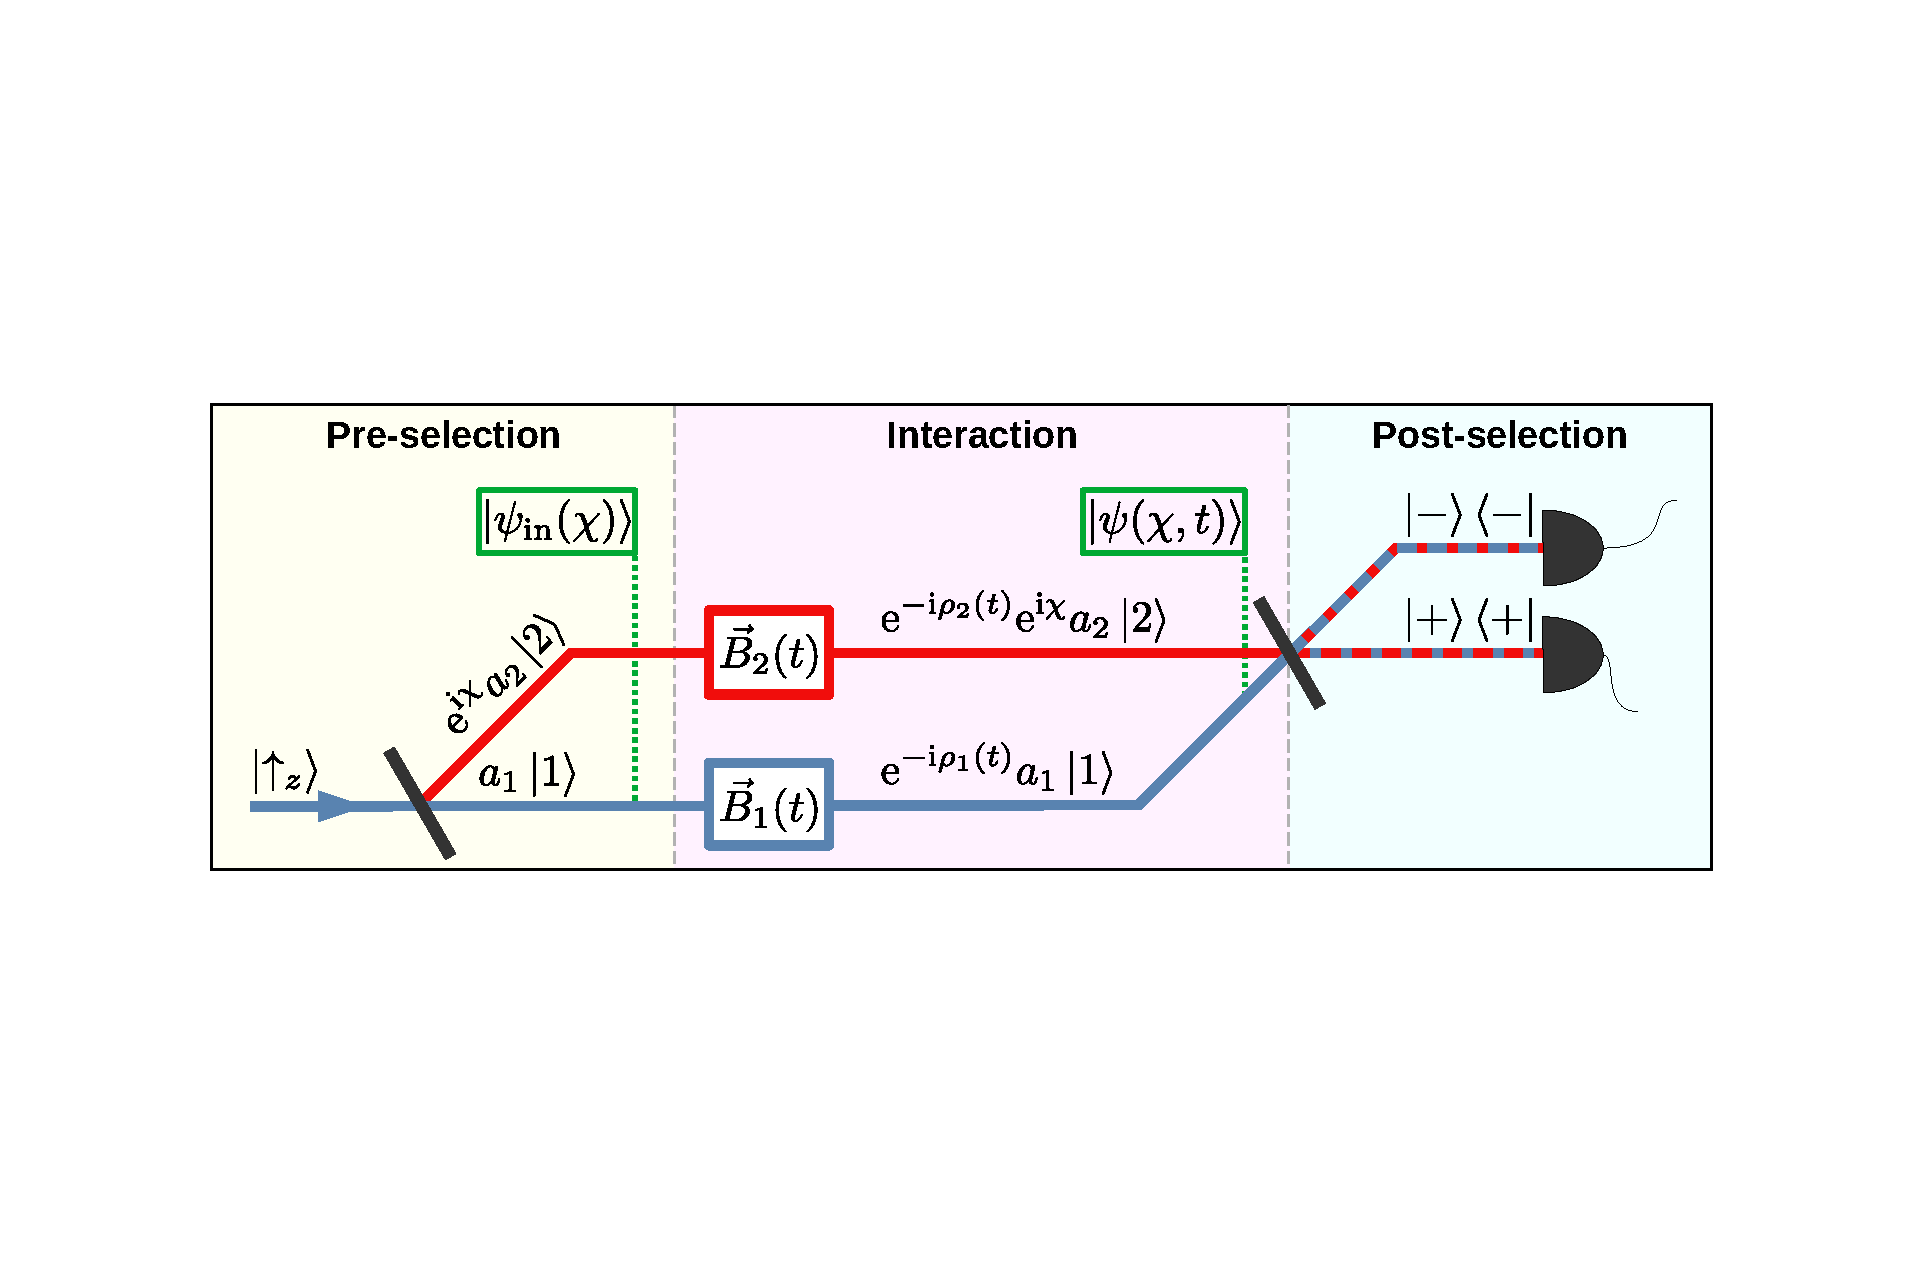
\includegraphics[width=0.95\linewidth,trim={3.5cm 6.5cm 3.5cm 6.5cm},clip]{Scheme theory.pdf}
\caption{\label{fig:inter_scheme} Scheme of an interferometer experiment with two oscillating magnetic fields generating time-dependent phases in each path. 
}
\end{figure}
\section{Theory}\label{sec:Theory}
\subsection{Neutron interferometry with oscillating magnetic fields}\label{subsec:interferometry}
Let us consider an interferometry scheme as the one shown in \fig\,\ref{fig:inter_scheme}, where a neutron polarised in the spin-up state $\ket{\uparrow_z}$ along the $z$-direction traverses a Mach-Zehnder interferometer. In each arm of the interferometer we place an oscillating magnetic field of the form $\Vec{B}_i(t)= 
        \left(0, 0, B_i\cos(\omega_i t + \varphi_i) \right),$
with $i=1,2$ indicating the path in which the field is present. The terms $\omega_i$ and $\varphi_i$ correspond to the angular frequency and phase of the oscillating field, respectively. Note that the magnetic fields involved are oriented in the $z$-direction, parallel to the spin state, and therefore no spin-flip is involved 
in the present case; the spinor part is constant and only the spacial wave-function evolves.

As the neutron enters the interferometer, it is put in an initial superposition of path states $\ket{1}$ and $\ket{2}$:
\begin{align}
    \ket{\psi_\mathrm{in}(\chi)}= a_1 
    \ket{1} +
    \e^{\I \chi}a_2 \ket{2} \,,
    \label{eq:psi_i}
\end{align}
with the path amplitudes $a_1$ and $a_2$ fulfilling $a_1^2+a_2^2=1$, and a relative phase $\chi$. Afterwards, the neutron interacts with the oscillating magnetic fields and the initial state acquires the following time-dependent phases\,\cite{summhammer1995,summhammer1993, sulyok2011, Haavig1982} (see \ref{app:time-phase}):
\begin{align}
\begin{aligned}
    \ket{\psi(\chi,t)} &= \e^{-\I \rho_1(t)} a_1 
    \ket{1} +
   \e^{-\I \rho_2(t)} \e^{\I \chi} a_2 \ket{2} \, ,
\end{aligned} \label{eq:psi}
\end{align}
with
\begin{align}
    \rho_i(t)=\alpha_i \sin(\omega_i t+\xi_i)\,,
    \label{eq:rho_i}
\end{align}
where
\begin{align}
    \alpha_i= 2\dfrac{\mu B_i}{\hbar \omega_i} \sin\left(\frac{\omega_i T_i}{2}\right) \, 
\qquad \mathrm{and} \qquad
        \xi_i&=\varphi_i+\frac{\omega_i T_i+\pi}{2}-\frac{\omega_i}{v_0}x \, .
    \label{eq:alpha xi}
\end{align}
The value $T_i$ corresponds to the interaction time, being the propagation time of the neutron in the oscillating field region, and $v_0$ is the neutron velocity in free space. 

The state $\ket{\psi(\chi,t)}$ represents the neutron's path wave-function after the interaction with the magnetic fields, right before the projection onto the states $\ket{+}$ and $\ket{-}$ from \eq\,\eqref{eq:+-}. The intensities at the two exit beams are given by the amplitude squared of the corresponding projections, via the relation
\begin{align}
\begin{aligned}
    I_{\pm}(\chi,t)&=\left|\braket{\pm|\psi(\chi,t)} \right|^2 = \frac{1}{2}\pm a_1 a_2 \cos(\chi+\rho_1(t) - \rho_2(t)) \, .
\end{aligned} \label{eq:I+-}
\end{align}
Note that the transformation $\ket{+} \rightarrow \ket{-}$ is equivalent to $\chi \rightarrow \chi\pm\pi$. Theoretical predictions of the time-dependent intensity $I_+(\chi,t)$ at different values of $\chi$ are shown in \fig\,\ref{fig:time_sim}. Here, intensity modulations generated by the time-dependent phases are visible. Such curves can be obtained via time-resolved measurements of the neutron counts, enabling the study of the time-dependent phases acquired by a neutron interacting with an oscillating magnetic field. 

We define the time-averaged intensity measured in the interval $(t_1,t_2)$, with an acquisition time $\tau=t_2-t_1$, as
\begin{align}
\begin{aligned}
    \braket{I_+(\chi, t)}_{\tau} &= \frac{1}{\tau} \int_{t_1}^{t_2} I_\pm(\chi,t) \mathrm{d}t \\&=\frac{1}{2} \pm \frac{a_1 a_2}{\tau} \sum_{n,m=-\infty}^\infty J_n(\alpha_1)J_m(\alpha_2) \int_{t_1}^{t_2} \cos(\chi +\omega_{nm} t + \xi_{nm})
     \, \mathrm{d}t \,,
\end{aligned}\label{eq:int I+-}
\end{align}
with $\omega_{nm}=n \omega_1 - m \omega_2$, $\xi_{n,m}=n \xi_1 - m \xi_2$, and $J_n(\cdot)$ being the $n$-th Bessel function of the first kind. In the case of only one coil being active and for a sufficiently long acquisition time $\tau_\infty\rightarrow\infty$, \eq\,\eqref{eq:int I+-} reduces to
\begin{align}
\begin{aligned}
    &\braket{I_\pm(\chi, t)}_{\tau\rightarrow\infty} = \frac{1}{2} \pm a_1 a_2 J_0(\alpha_i) \cos \chi \, ,
\end{aligned}\label{eq:int_I+-_T_inf}
\end{align}
with $i$ indicating the path in which the coil stays on. A step-by-step derivation of the analytical solutions of \eq\,\eqref{eq:int I+-} and \eq\,\eqref{eq:int_I+-_T_inf} can be found in \ref{app:time-avg}.
\begin{figure}[t]
\centering
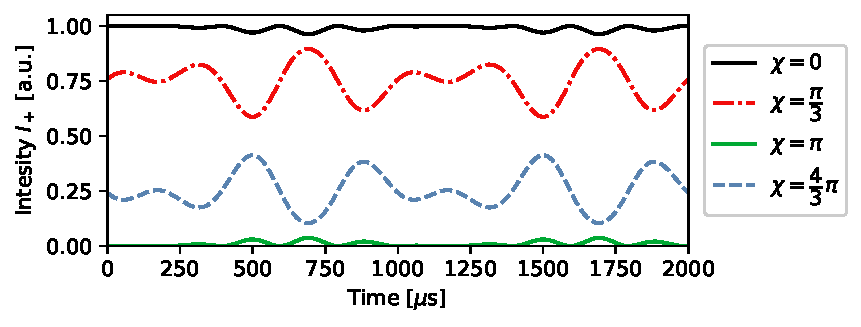
\includegraphics[width=0.8\linewidth,trim={0cm 0.25cm 0cm 0.25cm},clip]{time resolved sim.pdf}
\caption{\label{fig:time_sim} Time-dependent intensity $I_+$ for different values of $\chi$, with $\alpha_1=\alpha_2=\pi/16$, $\omega_1 = 4\pi\cdot10^{3} \,$rad/s, and $\omega_2 = 6 \pi \cdot 10^{3}\,$rad/s.}
\end{figure}
\subsection{Simultaneous measurement of the imaginary part of both path weak values}
Our goal is to extract information about the path weak values using the setup presented in 
Subsec.\,\ref{subsec:interferometry}. The path weak values $w_{\pm,i}$, with $i=1,2$, are complex quantities dependent on $\chi$ defined as
\begin{align}
    w_{\pm,i}(\chi) = \frac{\braket{\pm|\hat{\Pi}_i|\psi_\mathrm{in}(\chi)}}{\braket{\pm|\psi_\mathrm{in}(\chi)}} = w^\Re_{\pm,i}(\chi)+\I\, w^\Im_{\pm,i}(\chi) \, , \label{eq:wv}
\end{align}
where the terms $w^\Re_{\pm,i}$ and $w^\Im_{\pm,i}$ correspond to the real and imaginary part of the weak value, respectively. The state $\ket{\psi_\mathrm{in}(\chi)}$ presented in \eq\,\eqref{eq:psi_i}, the projectors $\hat{\Pi}_i = \ket{i}\bra{i}$, and the states $\ket{\pm}$ from \eq\,\eqref{eq:+-}, represent the pre-selection, the path observable to be measured, and the post-selections, respectively. 

Weak measurements are usually described in terms of von Neumann interaction, with a pointer state that is weakly coupled to a target system\,\cite{jozsa2007}. However, in the present scheme we consider the time-dependent phases $\rho_i(t)$ as parameters associated with the path projectors $\hat{\Pi}_i$ and the state in \eq\,\ref{eq:psi} can be expressed as:
\begin{align}
\begin{aligned}
    \ket{\psi(\chi,t)} &= \e^{-\I\left[ \rho_1(t)\hat{\Pi}_1+ \rho_2(t)\hat{\Pi}_2\right]}\ket{\psi_\mathrm{in}(\chi)}\, .
\end{aligned} \label{eq:psi_proj}
\end{align}
Despite not presenting the usual formalism of a weak measurement, experiments have been carried out considering a variable coupled to the target observable in place of a quantum meter, still maintaining a weak interaction\,\cite{kedem2014}. Furthermore, the absence of a quantum meter to be analyzed can be experimentally beneficial. The weakness of the coupling ensures that the state is minimally disturbed during the interaction. In our case the interaction strength is controlled by $\alpha_i$, which defines the maximum amplitude of the time-dependent phase. By choosing $\alpha$ appropriately, we can Taylor expand $\ket{\psi(\chi,t)}$ in powers of $\rho_1(t)$ and $\rho_2(t)$ and consider the weak limit, in which only the first order terms give a meaningful contribution and the higher orders are neglected. The projection on the $\ket{\pm}$ states then takes the form:
\begin{align}
\begin{aligned}
    \braket{\pm|\psi(\chi,t)} &\approx \bra{\pm}\left[1 -  \I \rho_1(t)\hat{\Pi}_1 -  \I \rho_2(t) \hat{\Pi}_2 \right] \ket{\psi_\mathrm{in}(\chi)} \\ 
    &= \braket{\pm|\psi_\mathrm{in}(\chi)}\left[1 -  \I \rho_1(t)w_{\pm,1} - \I \rho_2(t)w_{\pm,2} \right]\, , 
\end{aligned} \label{eq:+-psi_proj}
\end{align}
and the corresponding intensity is 
    \begin{align}
    \begin{aligned}
         I_\pm(\chi, t) &\approx  \lvert\braket{\pm|\psi_\mathrm{in}(\chi)}\rvert^2 \left[1 + 2\, w^\Im_{\pm,1}\, \rho_1(t) +  2\, w^\Im_{\pm,2}\, \rho_2(t)\right] \, ,
    \end{aligned} 
    \label{eq:+-I_weak}
\end{align}
with
\begin{align}
    \lvert \braket{\pm|\psi_\mathrm{in}(\chi)} \rvert^2 = \frac{1}{2} \pm 
    a_1a_2\cos\chi \, .
\end{align}
This result shows that the imaginary part of both path weak values can be simultaneously extracted from a weak measurement performed with the scheme shown in \fig\,\ref{fig:inter_scheme}. This scheme can be extended to an arbitrary number of paths by marking each path with additional time dependent phases $\rho_i(t)$.
\subsection{Extraction of the real part of the weak values}\label{subsec:real_part}
The weak values relative to the two post-selected states $\bra{+}$ and $\bra{-}$ obey the following equations:
\begin{align}
    w_{-,1}(\chi) &=  \frac{\braket{+|\psi_\mathrm{in}(\chi)}}{\braket{-|\psi_\mathrm{in}(\chi)}} w_{+,1}(\chi) \, , \ 
    w_{-,2}(\chi) = -\frac{\braket{+|\psi_\mathrm{in}(\chi)}}{\braket{-|\psi_\mathrm{in}(\chi)}} w_{+,2}(\chi) \label{eq:w-12}\, .
\end{align}
The ratio $\braket{+|\psi_\mathrm{in}(\chi)}/\braket{-|\psi_\mathrm{in}(\chi)}$ can be expressed in polar coordinates as
\begin{align}
    \frac{\braket{+|\psi_\mathrm{in}(\chi)}}{\braket{-|\psi_\mathrm{in}(\chi)}} = M \e^{\I \theta} \, ,
\end{align}
with $M=\left| \braket{+|\psi_\mathrm{in}(\chi)}/\braket{-|\psi_\mathrm{in}(\chi)}\right|$ and $\theta$ being the relative phase between the states after the post-selections. Together with \eq\,\eqref{eq:w-12} we get
\begin{align}
\begin{aligned}
    & w^\Im_{-,1}(\chi) = M\bigl(w^\Re_{+,1}(\chi)\sin \theta + w^\Im_{+,1}(\chi) \cos \theta\bigr) \\
    \Rightarrow & w^\Re_{+,1}(\chi) = \frac{w^\Im_{-,1}(\chi)}{M\sin \theta} - w^\Im_{+,1}(\chi) \cotan \theta
\end{aligned}\label{eq:real1}
\end{align}
and
\begin{align}
\begin{aligned}
    &w^\Im_{-,2}(\chi) = - M\bigl(w^\Re_{+,2}(\chi)\sin \theta + w^\Im_{+,2}(\chi) \cos \theta\bigr)\\
    \Rightarrow & w^\Re_{+,2}(\chi) = - \frac{w^\Im_{-,2}(\chi)}{M\sin \theta} - w^\Im_{+,2}(\chi) \cotan \theta \, . 
\end{aligned}\label{eq:real2}
\end{align}
The values of the amplitude $M$ and the different $w^\Im_{\pm,k}$ can all be obtained from \eq\,\eqref{eq:+-I_weak}. The phase $\theta$ has been extensively studied in neutron interferometry using different methods of extraction\,\cite{hasegawa1996,Wagh1998, filipp2005}, and it takes the value
\begin{align}
    \theta=\arctan\left(\dfrac{2a_1a_2 \sin\chi  }{{a_1}^2-{a_2}^2}\right)\, . \label{eq:theta}
\end{align}
If this phase is known, \eq\,\eqref{eq:real1} and \eq\,\eqref{eq:real2} allow the simultaneous extraction of the real part of the weak values.
% \begin{figure*}[t]
% \centering
% \includegraphics[width=\linewidth,trim={2cm 4.8cm 2cm 5cm},clip]{Setup numbers.pdf}
% \caption{\label{fig:inter_setup}Schematic drawing of the interferometer setup, from the left: magnetic prism(1), guide field(2), neutron interferometer(3), phase shifter(4), Indium absorbers(5), Helmholtz coils(6), $\ket{-}$-beam neutron detector(7), $\ket{+}$-beam neutron detector(8).}
% \end{figure*}
\begin{figure*}[t]
\centering
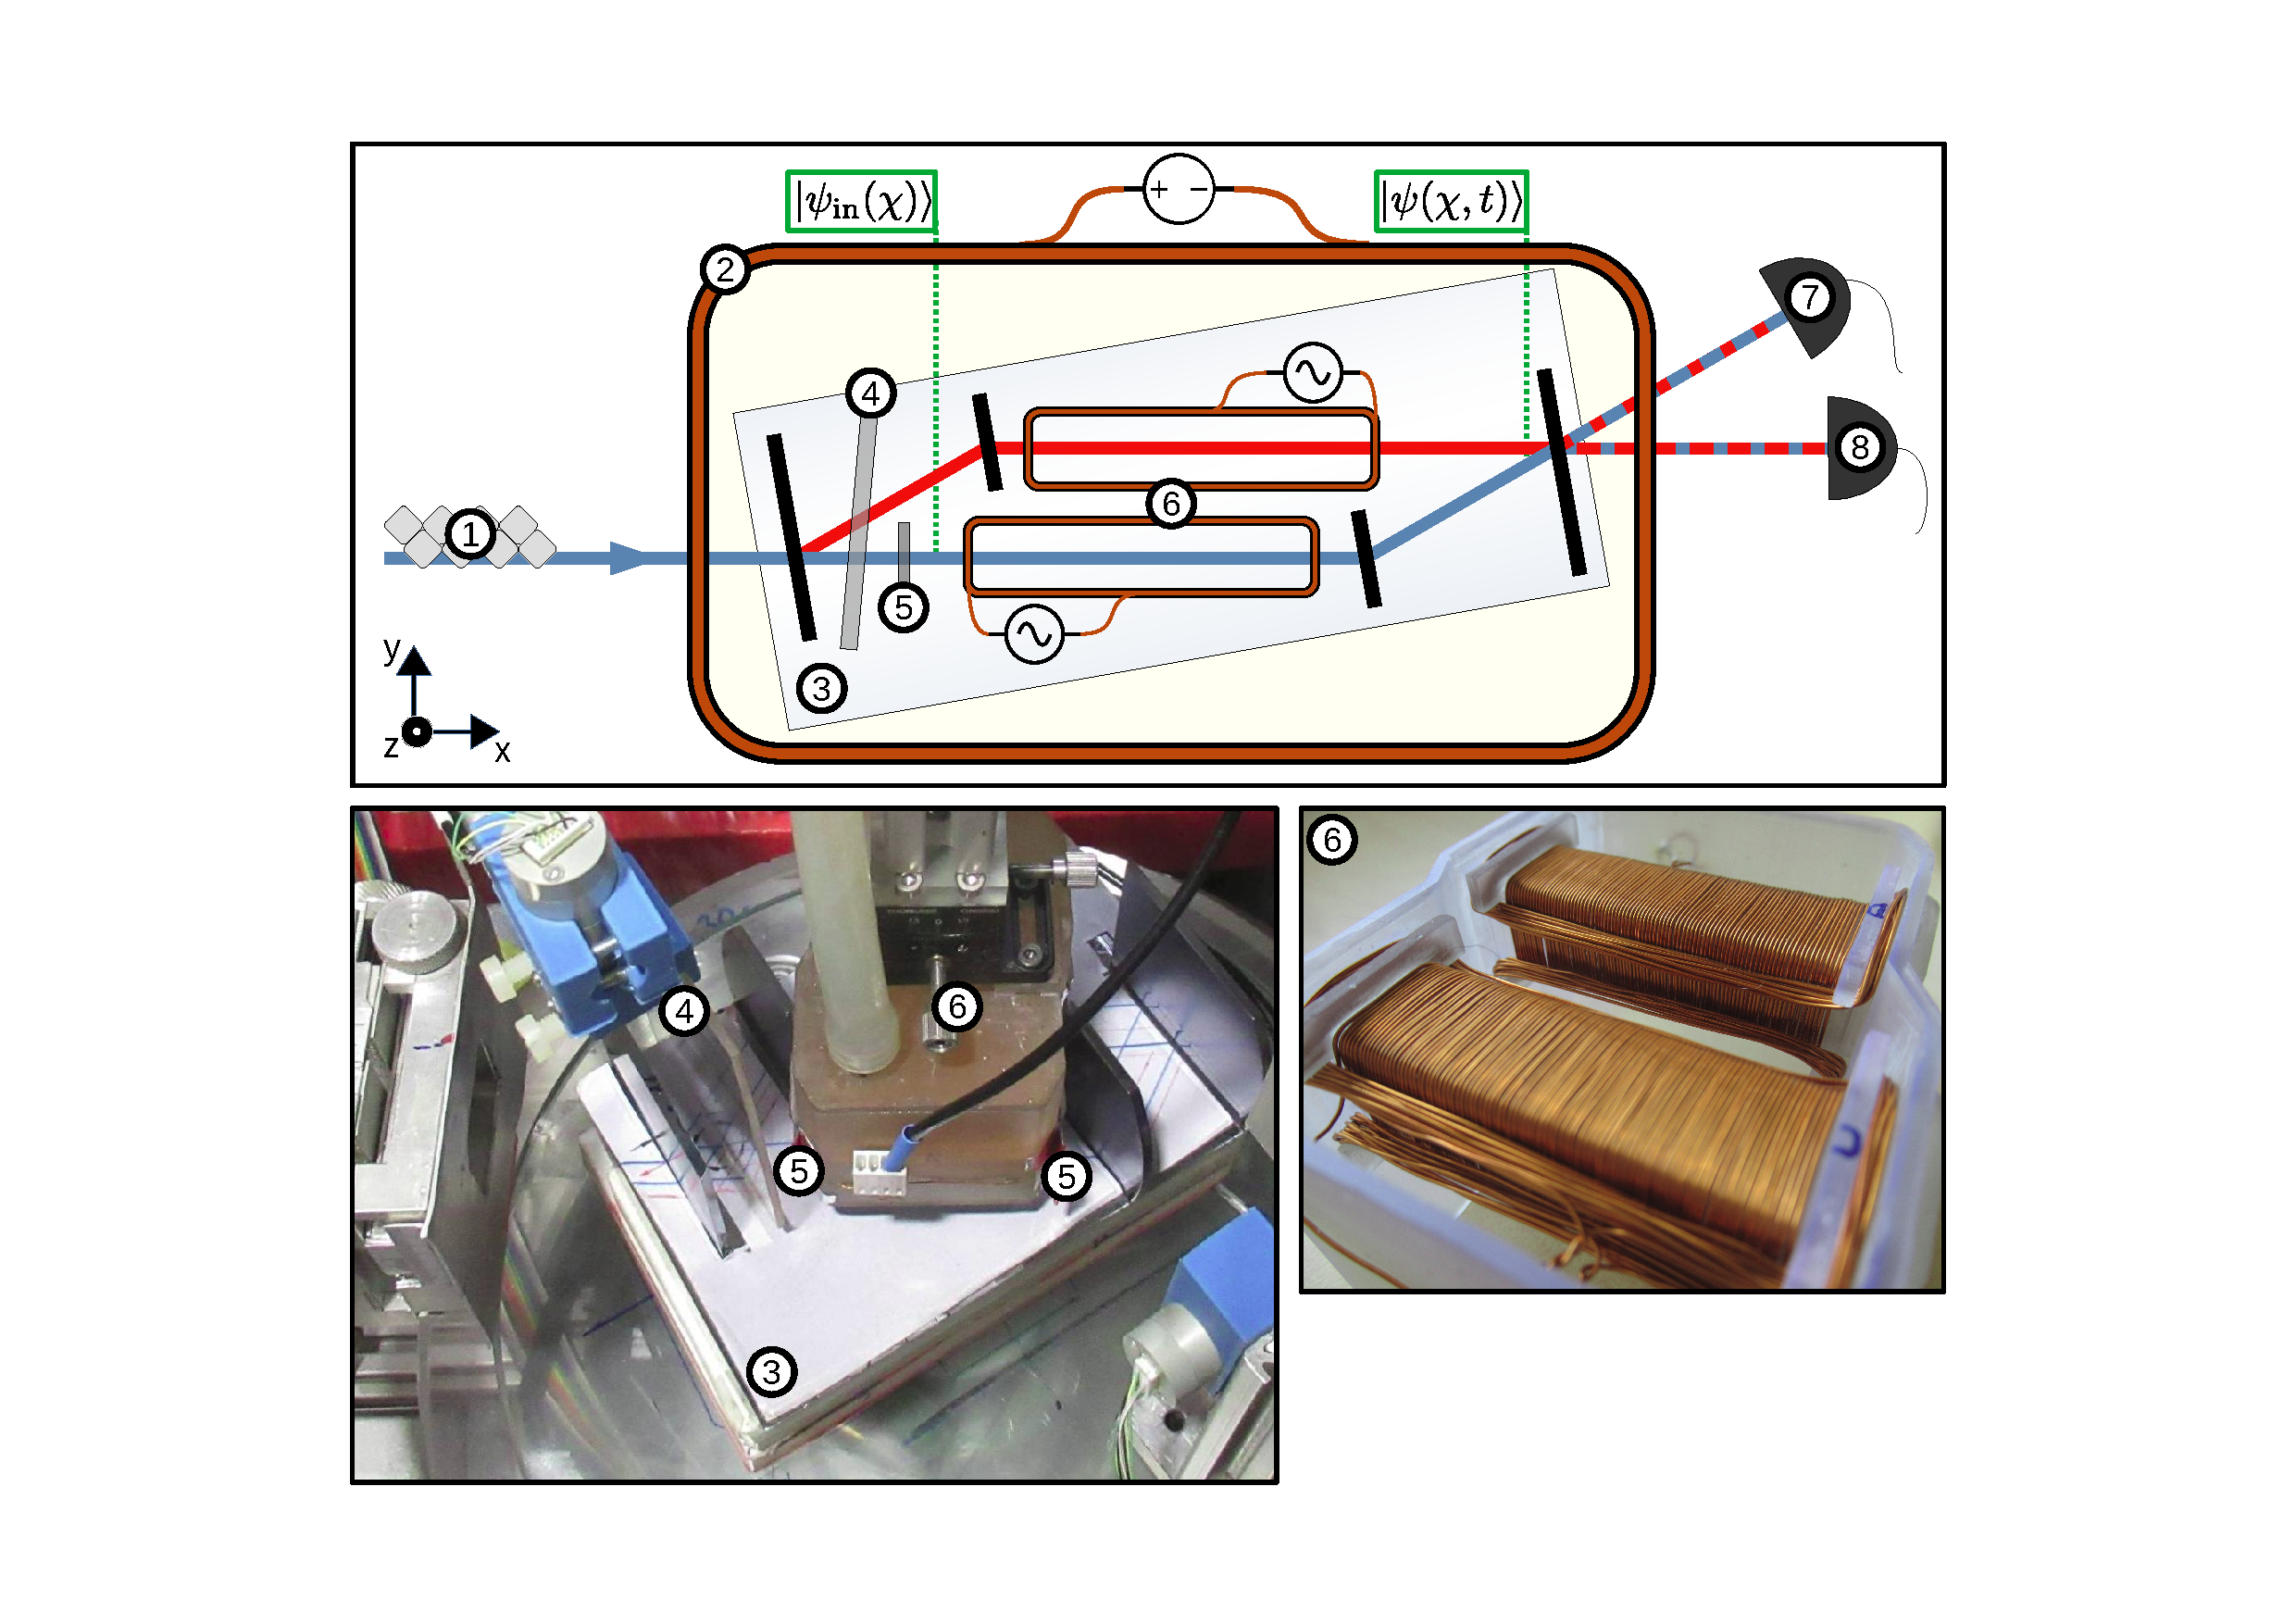
\includegraphics[width=\linewidth,trim={6.25cm 2.5cm 6.25cm 2.5cm},clip]{Setup numbers with pics.pdf}
\caption{\label{fig:inter_setup}Schematic drawing of the interferometer setup (top), with photos of the interferometer station (bottom left) and magnetic coils (bottom right). Setup elements: magnetic prism (1), guide field (2), neutron interferometer (3), phase shifter (4), Indium absorbers (5), Helmholtz coils (6), $\ket{-}$-beam neutron detector (7), $\ket{+}$-beam neutron detector (8).}
\end{figure*}
\section{Experiment}\label{sec:Exp}
\subsection{The setup}
The experiment was carried out at the instrument S18 of the Institut Laue-Langevin (ILL)\,\cite{geppert2014}, the setup is shown in \fig\,\ref{fig:inter_setup}. A neutron beam is monochromatised to a wavelength $\lambda=1.92$\,\AA, $\delta\lambda/\lambda\approx0.02$, and through a magnetic prism is polarised with a degree of polarisation $P>0.99$ in the vertical +$z$-direction, which defines the quantisation axis. In order to preserve polarisation, a constant magnetic field (guide field) is applied throughout the setup in the $z$-direction. The presence of the guide field does not affect the measurement results\,\cite{summhammer1993, sulyok2011}. The beam is split by the first plate of the single-crystal silicon neutron interferometer into two paths. A sapphire phase shifter (2.4 mm thickness) is placed in both paths of the interferometer, its rotation adjusts the relative phase $\chi$ between the paths. Measurements of the intensity for different phase shifter positions, usually referred to as interferograms, allow the adjustment of the desired relative phase.

Two indium foils of 1\,mm and 0.8\,mm thickness, with transmission coefficients of 47.1$\pm$0.3\% and 53.8$\pm$0.3\%, respectively, were used to control the path amplitudes $a_1$ and $a_2$. Generally, the path amplitudes are expected to be equal when no Indium is inserted, however, the measured ratio was $a_2/a_1 = 0.879 \pm 0.003$. This difference can be attributed to some damage of the interferometer, which was caused in a previous experiment and was fixed afterwards; the interferometer was chemically etched after a collision with an optical element. The measurements performed during the calibration stage exhibit good levels of phase homogeneity and contrast, the typical contrast for the different measurements is between 65\% and 75\% and the phase demonstrated good stability even for measurements with duration between 7 to 10 hours. The interferograms shown in \fig\,\ref{fig:ifg_phase_stability} were performed at different times of the same day, demonstrating the phase and contrast stability.
\begin{figure}[t]
\centering
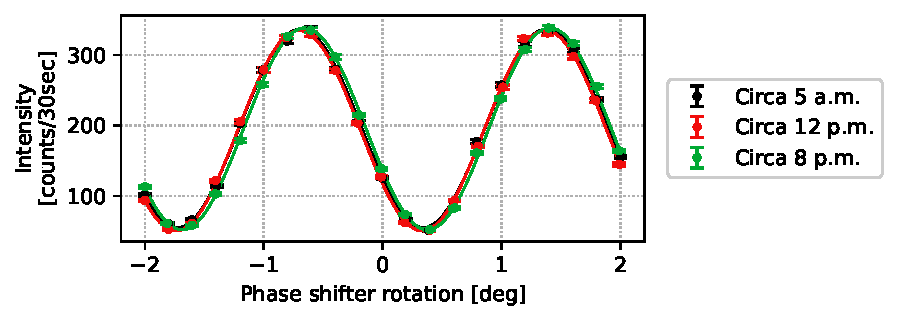
\includegraphics[width=0.9\linewidth,trim={0cm 0.2cm 0cm 0.2cm},clip]{Phase_stability.pdf}
\caption{\label{fig:ifg_phase_stability} Interferograms performed at different times of the same day demonstrating high stability in phase and contrast. Fits using a cosinusoidal function are shown with a continuous line.}
\end{figure}

In the interferometer, one Helmholtz coil\,\cite{danner2019} is placed in each path to generate the oscillating magnetic field parallel to the spin. The alignment of the magnetic field has been verified through spin analysis, as any misalignment would induce a spin rotation. Different spin orientations between paths would also reduce the contrast of the interferograms, which was used as an additional alignment indicator. The coils were water-cooled to prevent significant temperature changes which would affect the contrast and the phase stability. A skew-symmetric interferometer has been employed in order to maximize the longitudinal size of the coils ($\sim 50\,$mm), and consequently the time of flight of the neutron in the oscillating field region ($\sim 25\,\mu$s).

The last plate of the interferometer projects onto the states $\ket{+}$ and $\ket{-}$, associated with the interfering beams leaving in the forward and reflected direction, respectively. The neutron counts at the two exit ports are measured using $^3$He detectors. The time-resolved measurement is performed only on the $\ket{+}$-beam using a pencil detector of $\sim6$\,mm in diameter, with a time resolution of $\sim3\,\mu$s. As mentioned at the end of \sect\,\ref{sec:Theory} the results for the $\ket{-}$-beam can be retrieved by applying the transformation $\chi \rightarrow  \chi\pm\pi$ to the $\ket{+}$-beam. A major advantage of this setup is the absence of spin analysis, which is generally performed with a polarising multi-layer array, often referred to as supermirror. This optical element causes a significant loss of neutron counts up to one order of magnitude.
\subsection{Time-resolved measurements for different phase shifter positions}
\begin{figure}[t]
    \centering    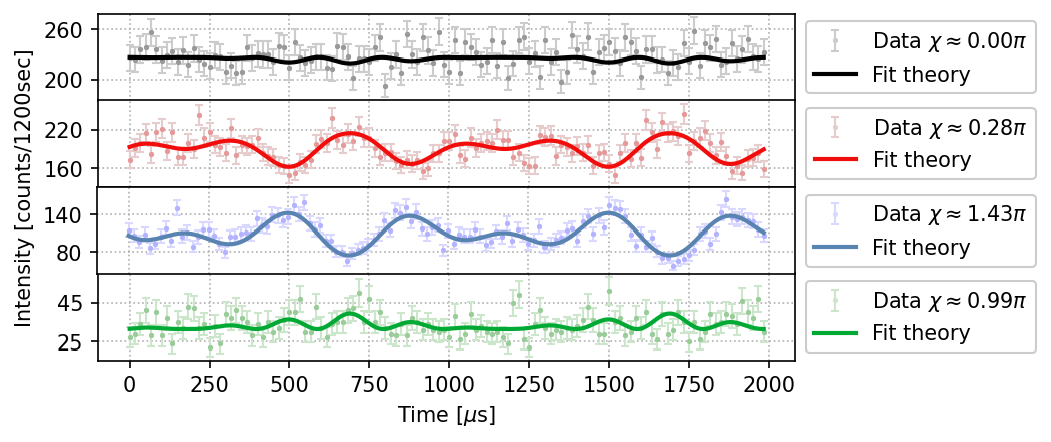
\includegraphics[width=\linewidth,trim={0cm 0.2cm 0cm 0.2cm},clip]{Measurement_example_fit.pdf}
    \caption{Typical time-dependent modulations of the intensity for different phase shifter positions $\chi$, with fitting of the data using \eq\,\eqref{eq:N}. The error-bars represent one standard deviation (Gaussian uncertainty).}
    \label{fig:meas_ex}
\end{figure}
A standard data set consists of time-resolved measurements performed at 22 different phase shifter positions. The frequencies used for the oscillating field in path 1 and path 2 were always 2 kHz (500\,$\mu$s period) and 3 kHz (333\,$\mu$s period), respectively. The frequencies were chosen in line with the characteristics of the coils, which define the interaction strength through the magnetic field and the interaction time, and the time resolution of the detector. Different frequencies might be used in different experimental contexts. The theoretical limit on the sampling frequency necessary to properly resolve the signal is imposed by the Nyquist-Shannon theorem\,\cite{shannon1949}; we sampled at $6\cdot 10^4$ points-per-second, way above the minimum sampling rate of $4\cdot 10^3$ points-per-second required by our lowest frequency, with a bin width of $\sim 16\,\mu$s. 

The time window for the measurement was chosen to be 1000\,$\mu s$ or 2000\,$\mu s$ to include one or two oscillation periods of the total signal, respectively. Each measurement has been acquired stroboscopically: exploiting the periodicity of the signal, the function generator would periodically trigger the detector to accumulate counts for the same oscillations over many repetitions. The total acquisition time was 1200\,s or 2000\,s for each phase shifter position. Typical time-resolved measurements relative to 4 different phase shifter positions are shown in Fig.\,\ref{fig:meas_ex}: the selected measurement are representative of the general characteristics of the time-oscillations and can be compared with the theoretical example of \fig\,\ref{fig:time_sim}. The most prominent oscillations occur for $\chi=\pm\pi/2$, an example of data in proximity of such a value is shown in \fig\,\ref{fig:time_avg}. The error-bars represent one standard deviation taken as the square root of the counts (Gaussian uncertainty). Here, it is possible to see the time-dependent oscillations arising from the phases generated by the oscillating magnetic fields.
\subsection{Measured neutron counts}
The description presented in \sect\,\ref{sec:Theory} is based on the idealised setup, but in order to extract the weak values from the experimental data the model has to include a contrast reduction due to imperfections of a real-life setup. In fact, a percentage of neutrons will not properly undergo path-interference generating an offset in the measured intensity. The non-interfering intensity $I_+^{\mathrm{N.I.}}$, i.e. the intensity without path interference, will receive contributions from both paths independently of $\chi$:
\begin{align}
\begin{aligned}
    I_+^{\mathrm{N.I.}} &= \lvert \braket{+|\hat{\Pi}_1|\psi(\chi,t)} \rvert^2 + \lvert \braket{+|\hat{\Pi}_2|\psi(\chi,t)} \rvert^2 = \frac{{a_1}^2+{a_2}^2}{2} = \dfrac{1}{2}\, ,
\end{aligned}
\end{align}
while the interfering components $I_+^{\mathrm{I.}}(\chi,t)$ will contribute to the total measured intensity proportionally to $I_+(\chi,t)$. The intensity measured at the detector $I^{\mathrm{D}}_+(\chi, t)$ can then be expressed as
\begin{align}
\begin{aligned}
        I^{\mathrm{D}}_+(\chi, t) &= A\left[(1-C)\,I_+^{\mathrm{N.I.}}+C\,I_+^{\mathrm{I.}}(\chi,t)\right] = A\left[(1-C)\frac{1}{2} + C \, I_+(\chi,t)\right]  ,
    \label{eq:N}
\end{aligned}
\end{align}
where $C$ is the percentage of fully interfering components and $A$ is a constant proportional to the neutron rate and the acquisition time. 

The time-averaged measured intensity is equal to
\begin{align}
\begin{aligned}
    \braket{I^{\mathrm{D}}_+(\chi, t)}_{\tau}&=\frac{1}{\tau} \int_{t_1}^{t_2} I^{\mathrm{D}}_+(\chi, t) \,\mathrm{d}t  = A\left(\frac{1-C}{2} + C\,  \braket{I_+(\chi,t)}_{\tau}\right) \, ,
\end{aligned} \label{eq:int Nc} 
\end{align}
which, using \eq\,\eqref{eq:int I+-}, in the case of $\alpha_1\approx\alpha_2\approx\pi/16$ can be approximated as 
\begin{align}
\begin{aligned}   
    \braket{I_+(\chi,t)}_{\tau} \approx \frac{1}{2} + a_1 a_2 \cos \chi \Rightarrow
    \braket{I^{\mathrm{D}}_+(\chi, t)}_{\tau}\approx A\left(\frac{1}{2} + C a_1 a_2 \cos \chi \right) \, .
\end{aligned} \label{eq:int_Nc_small_alpha} 
\end{align}
\begin{figure}[b]
    \centering    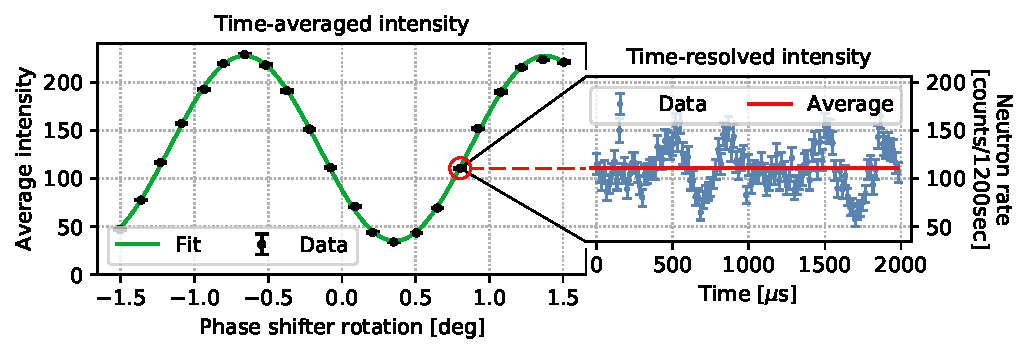
\includegraphics[width=\linewidth,trim={0.2cm 0cm 0.2cm 0cm},clip]{Time-average vs time-resolved.pdf}
    \caption{Time-averaged measurement for different phase shifter positions $\chi$, obtained from the time-resolved measurements, with fitting using \eq\,\eqref{eq:int_Nc_small_alpha}.}
    \label{fig:time_avg}
\end{figure}
The measured time-averaged intensity as presented in \eq\,\eqref{eq:int_Nc_small_alpha} is obtained directly by averaging the time-resolved measurements as shown in \fig\,\ref{fig:time_avg}, without the need for additional data. This allows the estimation of the proportionality constant $A$, appearing as the offset of the oscillation, and of the percentage of fully interfering components $C$, appearing as the contrast of the curve divided by $2 a_1 a_2$. Note that the time-averaged intensity of \fig\,\ref{fig:time_avg} is in all regards an interferogram and was used for the phase estimation in the weak value measurements. The measured time-averaged intensity with $\alpha_1\approx\alpha_2\approx\pi/16$ has been compared to the one with $\alpha_1=\alpha_2=0$: the measured contrast difference was $0.006 \pm 0.010$, confirming the validity of the approximation in \eq\,\eqref{eq:int_Nc_small_alpha}.
\subsection{Determination of the interaction strength}
The weak interaction is realized by adjusting the interaction strength $\alpha_i$, which could be in principle calculated using the magnetic field amplitude $B_i$ and the interaction time $T_i$, according to \eq\,\eqref{eq:alpha xi}. However, these parameters are difficult to determine, therefore a more direct experimental method is used. The interaction strength is directly proportional to the amplitude $B_i$ of the oscillating magnetic field, which is generated from an alternating current (AC) flowing in each coil. The AC is controlled by a function generator through an input voltage of amplitude $V_i$, being the adjustable parameter in the experiment. Hence, we have $\alpha_i \propto B_i \propto V_i$,
and the relation between $\alpha_i$ and $V_i$ has to be determined in order to be able to adjust the interaction strength experimentally. This can be achieved by measuring the time-averaged neutron counts for a sufficiently long acquisition time $\tau_\infty\rightarrow\infty$. Let us assume only one coil being active in one of the paths, in this case from \eq\,\eqref{eq:int_I+-_T_inf} and \eq\,\eqref{eq:int Nc} we get
\begin{align}
\begin{aligned}   
    \braket{I^{\mathrm{D}}_+(\chi, t)}_{\tau_\infty}=A\left(\frac{1}{2} + C a_1 a_2 J_0(\alpha_i) \cos \chi \right) 
\end{aligned} \label{eq:int_Nc_alpha_i} 
\end{align}
with $i$ indicating the path in which the coil is active.

For fixed values of $C$, $a_1$, and $a_2$, the contrast of the oscillations due to $\chi$ in \eq\,\eqref{eq:int_Nc_alpha_i} is proportional to $\left|J_0(\alpha_i)\right|$. Therefore by measuring such contrast for different input voltages, we can find the relation between $\left|\alpha_i\right|$ and $V_i$. For the sake of simplicity, we will assume $\alpha_i$ to be positive and the sign of $\rho_i$ can be defined by the phase $\xi_i$ from \eq\,\eqref{eq:rho_i}.

\begin{wrapfigure}{r}{0.5\textwidth}
\centering
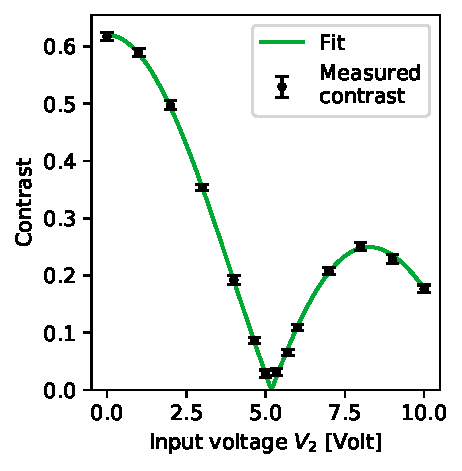
\includegraphics[width=0.9\linewidth,trim={0cm 0.2cm 0cm 0.2cm},clip]{Alpha_calibration_example.pdf}
\caption{\label{fig:ifg_vs_alpha} Example of calibration of $\alpha_2$ as a functions of the input voltage $V_2$, for $\omega_2=3$ kHz.}
\end{wrapfigure}
In our case, the oscillation period $2\pi/\omega_i$ is less than one millisecond for both coils and therefore any acquisition time above one second is a good approximation for $\tau_\infty$. Setting an acquisition time of 15 seconds, the oscillations predicted by \eq\,\eqref{eq:int_Nc_alpha_i} have been recorded for different values of $V_i$ and the contrast of the oscillations in $\chi$ has been extracted. Afterwards, the resulting values have been fitted with the function
\begin{align}
    F(V_i) = \mathbf{f_{0}}_{i}\, \left|J_0(\mathbf{f_{1}}_{i} V_i)\right| \,,
\end{align}
with $\mathbf{f_{0}}_{i}$ and $\mathbf{f_{1}}_{i}$ as fit parameters. An example of such a fit is shown in \fig\,\ref{fig:ifg_vs_alpha}. The interaction strength as a function of the input voltage is then obtained as $\alpha_i=\mathbf{f_{1}}_{i} V_i$. For the weak interaction, the values of $\alpha_i$ have been set to $\alpha_1 = 0.193 \pm 0.001$ and 
$\alpha_2 = 0.197 \pm 0.001$, i.e., approximately $\pi/16$. With such values of $\alpha_i$, the fidelity\,\cite{walls2008} between the initial state $\ket{\psi_\mathrm{in}(\chi)}$ and the state after the interaction $\ket{\psi(\chi)}$ is 
$F=\left|\braket{\psi_\mathrm{in}(\chi)|\psi(\chi,t)}\right|^2\gtrsim0.96$, confirming the weakness of the interaction.
\subsection{Weak values extraction from data}\label{subsec:WvExtrData}
According to \eq\,\eqref{eq:+-I_weak} and \eq\,\eqref{eq:N}, for sufficiently small $\alpha_1$ and $\alpha_2$  the intensity measured at the detector can be approximated as
\begin{align}
\begin{aligned}
    I^{\mathrm{D}}_+(\chi, t) &\approx
     A\bigg[\frac{1-C}{2} + C \, \lvert\braket{+|\psi_\mathrm{in}(\chi)}\rvert^2 \left(1 + 2\, w^\Im_{+,1}(\chi)\,\alpha_1 \sin\left( \omega_1 t + \xi_1\right)\right. \\&+ \left. 2\, w^\Im_{+,2}(\chi)\,\alpha_2 \sin\left( \omega_2 t+\xi_2\right)\,\right)\bigg] \, .
    \label{eq:N_weak}
\end{aligned}
\end{align}
The parameters $A$ and $C$ are determined using the time-averaged measured intensity according to \eq\,\eqref{eq:int_Nc_small_alpha}, while the imaginary part of the weak value can be experimentally derived from \eq\,\eqref{eq:N_weak} using two methods. The first method consists of fitting the measured intensity with a function $G(t)$ that includes an offset and two oscillating terms with angular frequencies $\omega_1$ and $\omega_2$:
\begin{align}
    G(t)= \mathbf{g_0}+2\,\mathbf{g_1} \sin\left( \omega_1 t + \mathbf{g_2}\right) + 2\,\mathbf{g_3} \sin\left(\omega_2 t+\mathbf{g_4}\right)\, ,
\end{align}
where $\mathbf{g_k}$ with $k=1,2,3,4$ are fit parameters. According to \eq~\eqref{eq:N_weak}, we have
\begin{align}
\begin{aligned}
    \mathbf{g_0}&=A(1-C)/2 + A \, C \, \lvert\braket{+|\psi_\mathrm{in}(\chi)}\rvert^2\, ,\
    \mathbf{g_1}=A \, C \, \lvert\braket{+|\psi_\mathrm{in}(\chi)}\rvert^2 w^\Im_{+,1}\, , \
    \mathbf{g_2}=\xi_1\, , \\
    \mathbf{g_3}&=A \, C \, \lvert\braket{+|\psi_\mathrm{in}(\chi)}\rvert^2 w^\Im_{+,2}\, , \ \ \mathrm{and}\ \
    \mathbf{g_4}=\xi_2\, .
\end{aligned}
\end{align}
The imaginary part of both path weak values can then be determined as
\begin{align}
         w^\Im_{+,1} = \frac{\mathbf{g_1}}{\alpha_1\left[\mathbf{g_0}-A(1-C)/2\right]} \qquad \mathrm{and} \qquad
         w^\Im_{+,2} = \frac{\mathbf{g_3}}{\alpha_2\left[\mathbf{g_0}-A(1-C)/2\right]}\, .\label{eq:Im_fit}
\end{align}
The error-bars are obtained from standard error propagation using the uncertainty on the fit parameters obtained from the covariance matrix of the fit. The second method employs the Fourier analysis of the measured intensity. The Fourier components
\begin{align}
    c_\omega= \int_{-\infty}^{\infty} e^{-\I \omega t}  I^{\mathrm{D}}_+(\chi, t) \, dt\label{eq:cw}
\end{align}
of equation \eq\,\eqref{eq:N_weak} are
\begin{align}
            c_0=A(1-C)/2 + A \, C \, \lvert\braket{+|\psi_\mathrm{in}(\chi)}\rvert^2 \ \ \mathrm{and} \ \
            c_{\omega_i}= A\, C \lvert\braket{+|\psi_\mathrm{in}(\chi)}\rvert^2 \alpha_i\,w^\Im_{+,i} \, \e^{\I (\xi_i-\frac{\pi}{2})} \, ,
\end{align}
yielding
\begin{align}
    \lvert\braket{+|\psi_\mathrm{in}(\chi)}\rvert^2 =\frac{1}{AC} \left(c_0-\dfrac{A(1-C)}{2}\right) \, 
\label{eq:cos2_Fourier}
\end{align}
and
\begin{align}
    w^\Im_{+,i} = \frac{c_{\omega_i}}{\left(c_0-\dfrac{A(1-C)}{2}\right)\alpha_i \e^{\I (\xi_i-\frac{\pi}{2})}} \, .
\label{eq:Im_Fourier}
\end{align}
The error-bars are obtained from standard error propagation using the following uncertainty on the Fourier components\,\cite{sulyok2011}:
\begin{align}
    \Delta(c_0) = \sqrt{\braket{I^{\mathrm{D}}_+(\chi, t)}} \qquad \mathrm{and} \qquad \Delta(c_{\omega_i}^\Re) = \Delta(c_{\omega_i}^\Im) = \sqrt{\frac{\braket{I^{\mathrm{D}}_+(\chi, t)}}{2}}\, . \label{eq:error_fourier}
\end{align}

In both methods there is an ambiguity in the sign of the imaginary part of the weak value due to the indefiniteness of $\xi_i$. Lifting this ambiguity is not necessary if one is interested in extracting the imaginary part of the path weak values up to a global sign. If needed, both $\xi_i$ can be determined from \eq\,\eqref{eq:alpha xi}, if the interaction time $T_i$ and the detector position are known, or, alternatively, they can be extracted by fitting a time-resolved measurement as the one in \fig\,\ref{fig:meas_ex}. The measurement of the phases $\xi_i$ should be performed only once and does not have to be repeated as long as the coils and the detector are kept at the same relative distance.
\section{Results}\label{sec:Res2}
\begin{figure}[t]
\centering
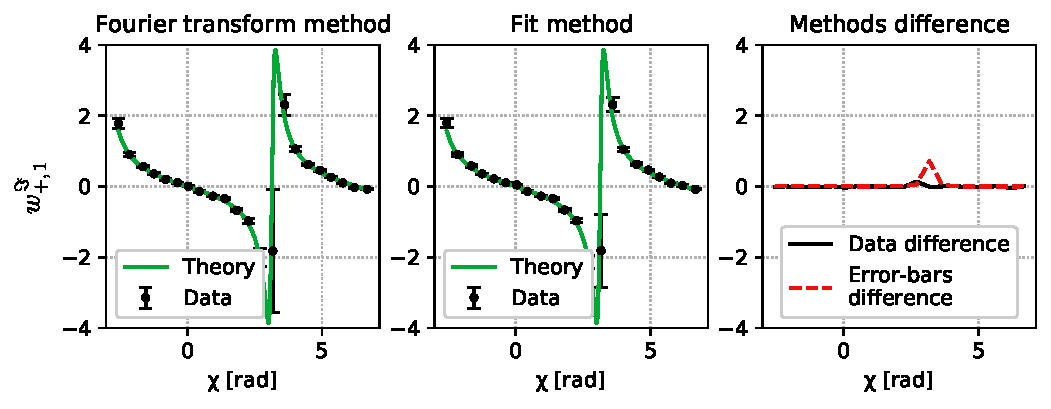
\includegraphics[width=\linewidth,trim={0.2cm 0.2cm 0.2cm 0.2cm},clip]{Fourier vs Fit.pdf}
\caption{Example of data extracted using \eq\,\eqref{eq:Im_Fourier} (left) and \eq\,\eqref{eq:Im_fit} (center). The difference between the resulting data points and resulting error-bars is plotted for better comparison (right).}\label{fig:Fourier vs fit}
\end{figure}
In this section we report the results of the simultaneous measurement of the path weak values. The interaction strengths have been set to 
$\alpha_1 = 0.193 \pm 0.001$ and 
$\alpha_2 = 0.197 \pm 0.001$, approximately $\pi/16$, for all measurements. The phase shifter has been used to adjust $\chi$, while Indium absorbers have been used to realize three different configurations of path amplitudes. The path amplitudes ratios were $a_2/a_1\approx1.75$, $a_2/a_1\approx1.20$, and $a_2/a_1\approx 0.88$, and the results for these three configuration are shown in \fig\,\ref{fig:results a21=1.75}, \ref{fig:results a21=1.20} and \ref{fig:results a21=0.88}, respectively. 

A comparison of the two methods of extraction presented in the previous section is shown in \fig\,\ref{fig:Fourier vs fit}, here it is possible to observe the difference between the resulting data and error-bars. The methods yield similar outputs, therefore we present only the results obtained using the Fourier analysis of the measured intensity. The imaginary part $w^\Im_{+,i}$ of the weak values is then obtained according to \eq\,(\ref{eq:cw}-\ref{eq:error_fourier}). The proportionality constant $A$ and the percentage of fully interfering components $C$ have been determined according to \eq\,\eqref{eq:int_Nc_small_alpha}. The real part $w^\Re_{+,i}$ of the weak value is extracted according to \eq\,\eqref{eq:real1} and \eqref{eq:real2}. The values of $w^\Im_{-,i}$ are obtained by shifting the data points of $w^\Im_{+,i}$ according to $\chi\rightarrow\chi\pm\pi$, while the phase $\theta$ is assumed to be known with values derived from \eq\,\eqref{eq:theta}. To further highlight the validity of the experimentally derived weak values, the sums of their components $w^\Im_{+,1}+w^\Im_{+,2}=0$ and $w^\Re_{+,1}+w^\Re_{+,2}=1$ are shown. The results are compared to the theoretical curves obtained from the explicit form of \eq\,\eqref{eq:wv}:
\begin{align}
    w_{\pm,1}(\chi) = \frac{1}{1\pm \frac{a_2}{a_1}\e^{\I \chi}} \qquad \mathrm{and} \qquad
    w_{\pm,2}(\chi) = \frac{1}{\frac{a_1}{a_2}\e^{-\I \chi}\pm1}\, .
\end{align}

\begin{figure}[t]
\centering
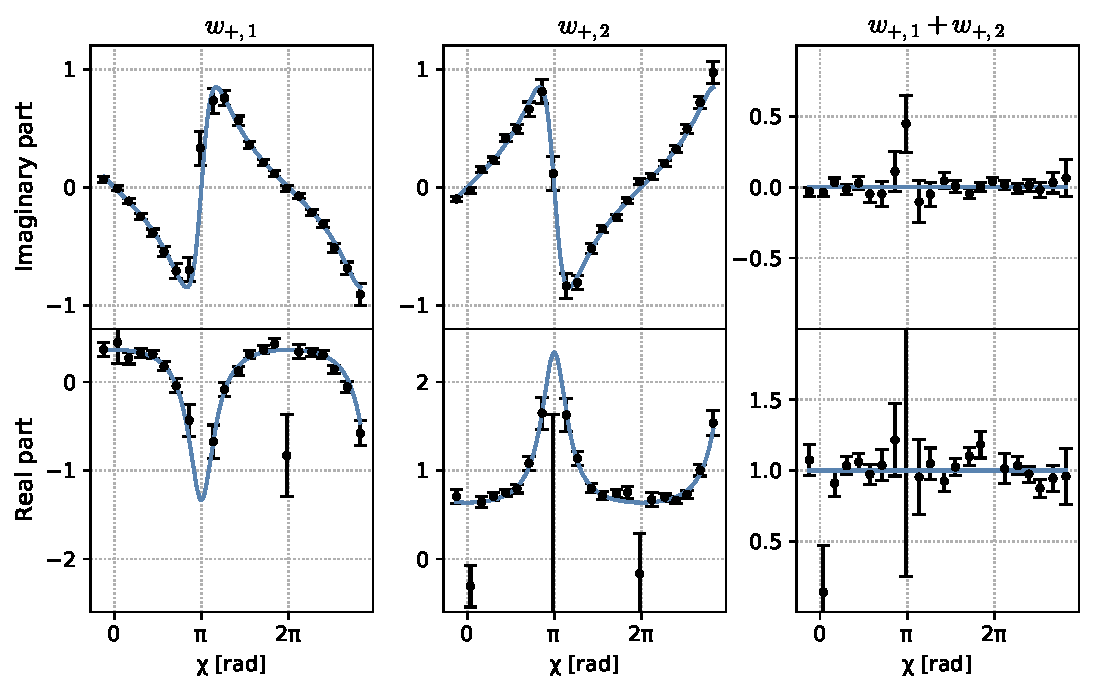
\includegraphics[width=0.98\linewidth,trim={0cm 0.25cm 0cm 0.25cm},clip]{Wv In 1p8 combined.pdf}
\caption{\label{fig:results a21=1.75} Resulting weak values (data points) compared with the theoretical prediction (continuous line) for $\alpha_1 \approx \alpha_2 \approx \pi/16$ and $a_2/a_1\approx 1.75$, plotted as their real and imaginary part for the different values of $\chi$.
}
\end{figure}
The experimental results for the imaginary part of both path weak values are in good agreement with the theory. When the curve gets particularly steep in the vicinity of $\chi=\pm\pi$, the measurements get more sensitive to small phase instabilities. This can result in the error-bars getting larger with the steepness of the slope, as it is clearly observable in \fig\,\ref{fig:results a21=1.20} and \ref{fig:results a21=0.88}, and in a significant deviation from the theoretical prediction for $w^\Im_{+,1}+w^\Im_{+,2}$. Another factor contributing to the size of the error-bars around $\chi=\pm\pi$ is the neutron counts approaching the minimum, resulting in an increased relative Gaussian uncertainty. The experimental results for the real part are also in good agreement with the theory, however they present some important criticality around $\chi=0,\pm\pi$. The large error-bars near $\chi=\pm\pi$, distinctly
noticeable \fig\,\ref{fig:results a21=1.20} and \ref{fig:results a21=0.88}, are a direct consequence of the large error-bars of the imaginary parts that were used to derive these results. The points approaching $\chi=0,\pm\pi$ significantly deviate from the theory curve, sometimes exceeding the y-axis range. For the sake of clarity, the plot range has not been extended to the most distant outliers. The deviation of the data is attributed to \eq\,\eqref{eq:real1} and \eq\,\eqref{eq:real2} diverging for those values of $\chi$, if the measured $w^\Im_{+,i}$ and $w^\Im_{-,i}$ do not go to 0 as predicted by the theory. This divergence can extremely amplify small fluctuations in the data, explaining the significant discrepancy.
\begin{figure}[t]
\centering
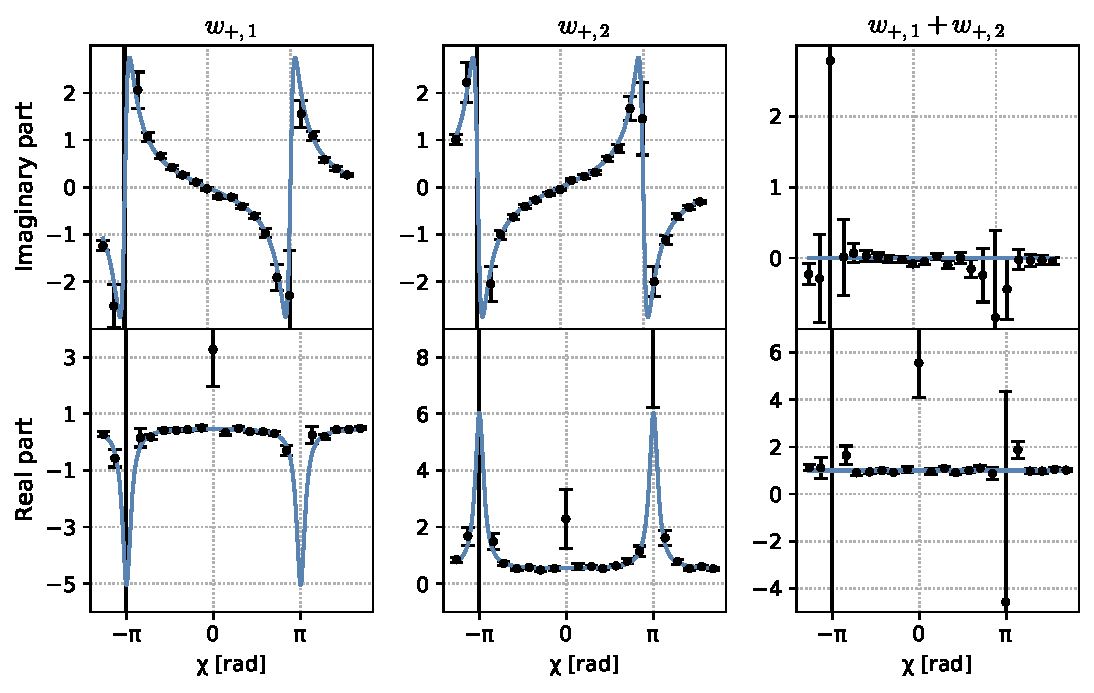
\includegraphics[width=0.98\linewidth,trim={0cm 0.2cm 0cm 0.2cm},clip]{Wv In 0p8 combined.pdf}
\caption{\label{fig:results a21=1.20} Resulting weak values (data points) compared with the theoretical prediction (continuous line) for $\alpha_1 \approx \alpha_2 \approx \pi/16$ and $a_2/a_1\approx 1.20$, plotted as their real and imaginary part for the different values of $\chi$. 
}
\end{figure}
\begin{figure}[t]
\centering
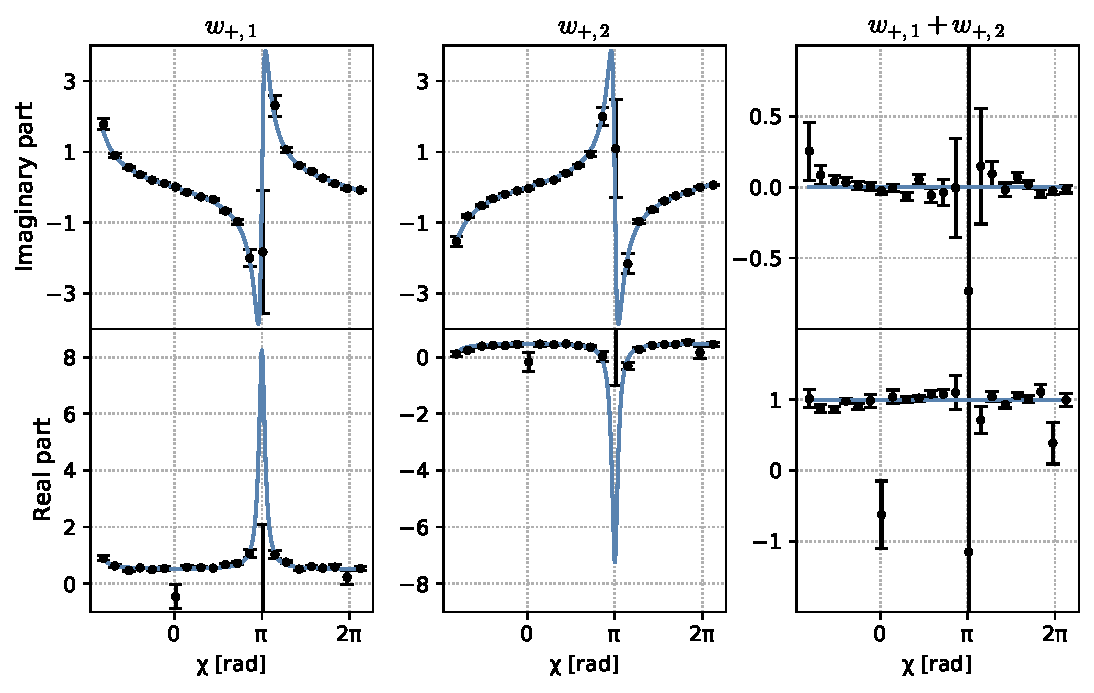
\includegraphics[width=\linewidth,trim={0cm 0.25cm 0cm 0.25cm},clip]{Wv No In combined.pdf}
\caption{\label{fig:results a21=0.88} Resulting weak values (data points) compared with the theoretical prediction (continuous line) for $\alpha_1 \approx \alpha_2 \approx \pi/16$ and $a_2/a_1\approx 0.88$, plotted as their real and imaginary part for the different values of $\chi$.
}
\end{figure}
\section{Conclusion}\label{sec:Disc}
We presented a neutron interferometer experiment with time-dependent manipulation, which allows the simultaneous extraction of the imaginary parts of both path weak values without the need for spin analysis. We have also demonstrated a relation among the real part of a path weak value, its imaginary part, and the imaginary part of the weak value relative to the alternative orthogonal post-selected state. This relation allows the additional simultaneous extraction of the real part of both path weak values, provided that the relative phase between $\braket{+|\psi(\chi)}$ and $\braket{-|\psi(\chi)}$ is known. 

The results for the simultaneously extracted imaginary part are in good agreement with the theory, confirming the effectiveness of the scheme. The results for the real part of the weak values are overall in agreement with the theory, except for the points around $\chi=0$ and $\chi=\pm\pi$. For those specific values, some terms in \eq\,\eqref{eq:real1} and \eq\,\eqref{eq:real2} tend to diverge and therefore small fluctuations in the imaginary part of the weak value can be extremely amplified resulting in a significant deviation of the data from the theoretical values.
\section{Acknowledgements}
This research was funded in part by the Austrian Science Fund (FWF) [grant DOI: 10.55776/P34105]. For open access purposes, the authors have applied a CC BY public copyright license to any authors accepted manuscript version arising from this submission. The authors acknowledge the hospitality of ILL, the data that support the findings of this study are available at the following DOI: 10.5291/ILL-DATA.CRG-3061. The authors acknowledge TU Wien Bibliothek for financial support through its Open Access Funding Program.
\appendix
\section{Time-dependent phase generation with oscillating magnetic fields}\label{app:time-phase}
Let us consider a magnetic field oriented in the $z$-direction of the form $\Vec{B}=(0,0,B_z(x))$, as the one shown in \fig\,\ref{fig:B field}, with
\begin{align}
\begin{aligned}
    \begin{cases}
        B_z(x)=0 \ &\mathrm{for} \ |x|>L  \\
        B_z(x)=B \cos(\omega t + \varphi) \ &\mathrm{for} \ |x|\leq L
    \end{cases} \, ,
\end{aligned}
\end{align}
The non-relativistic interaction between a neutron polarised along the $z$-direction in the spin-up state $\ket{\uparrow_z}$ and such a magnetic field is described by the Schrödinger-Pauli (SP) equation\,\cite{Pauli1988}
\begin{align}
    \I \hbar \frac{\partial}{\partial t} \ket{\psi(t)} = \left[\frac{\hat{p}^2}{2m}+\mu\, \hat{\Vec{\sigma}} \cdot \Vec{B} \right] \ket{\psi(t)} \Rightarrow \I \hbar \frac{\partial}{\partial t} \psi(x,t) = \left[\frac{\hbar^2}{2m}\frac{\partial^2}{\partial x^2}+\mu\, B_z(x) \right] \psi(x,t)\,,
    \label{eq:P-S-B-up-x}
\end{align}
\begin{wrapfigure}{r}{0.45\textwidth}
\centering
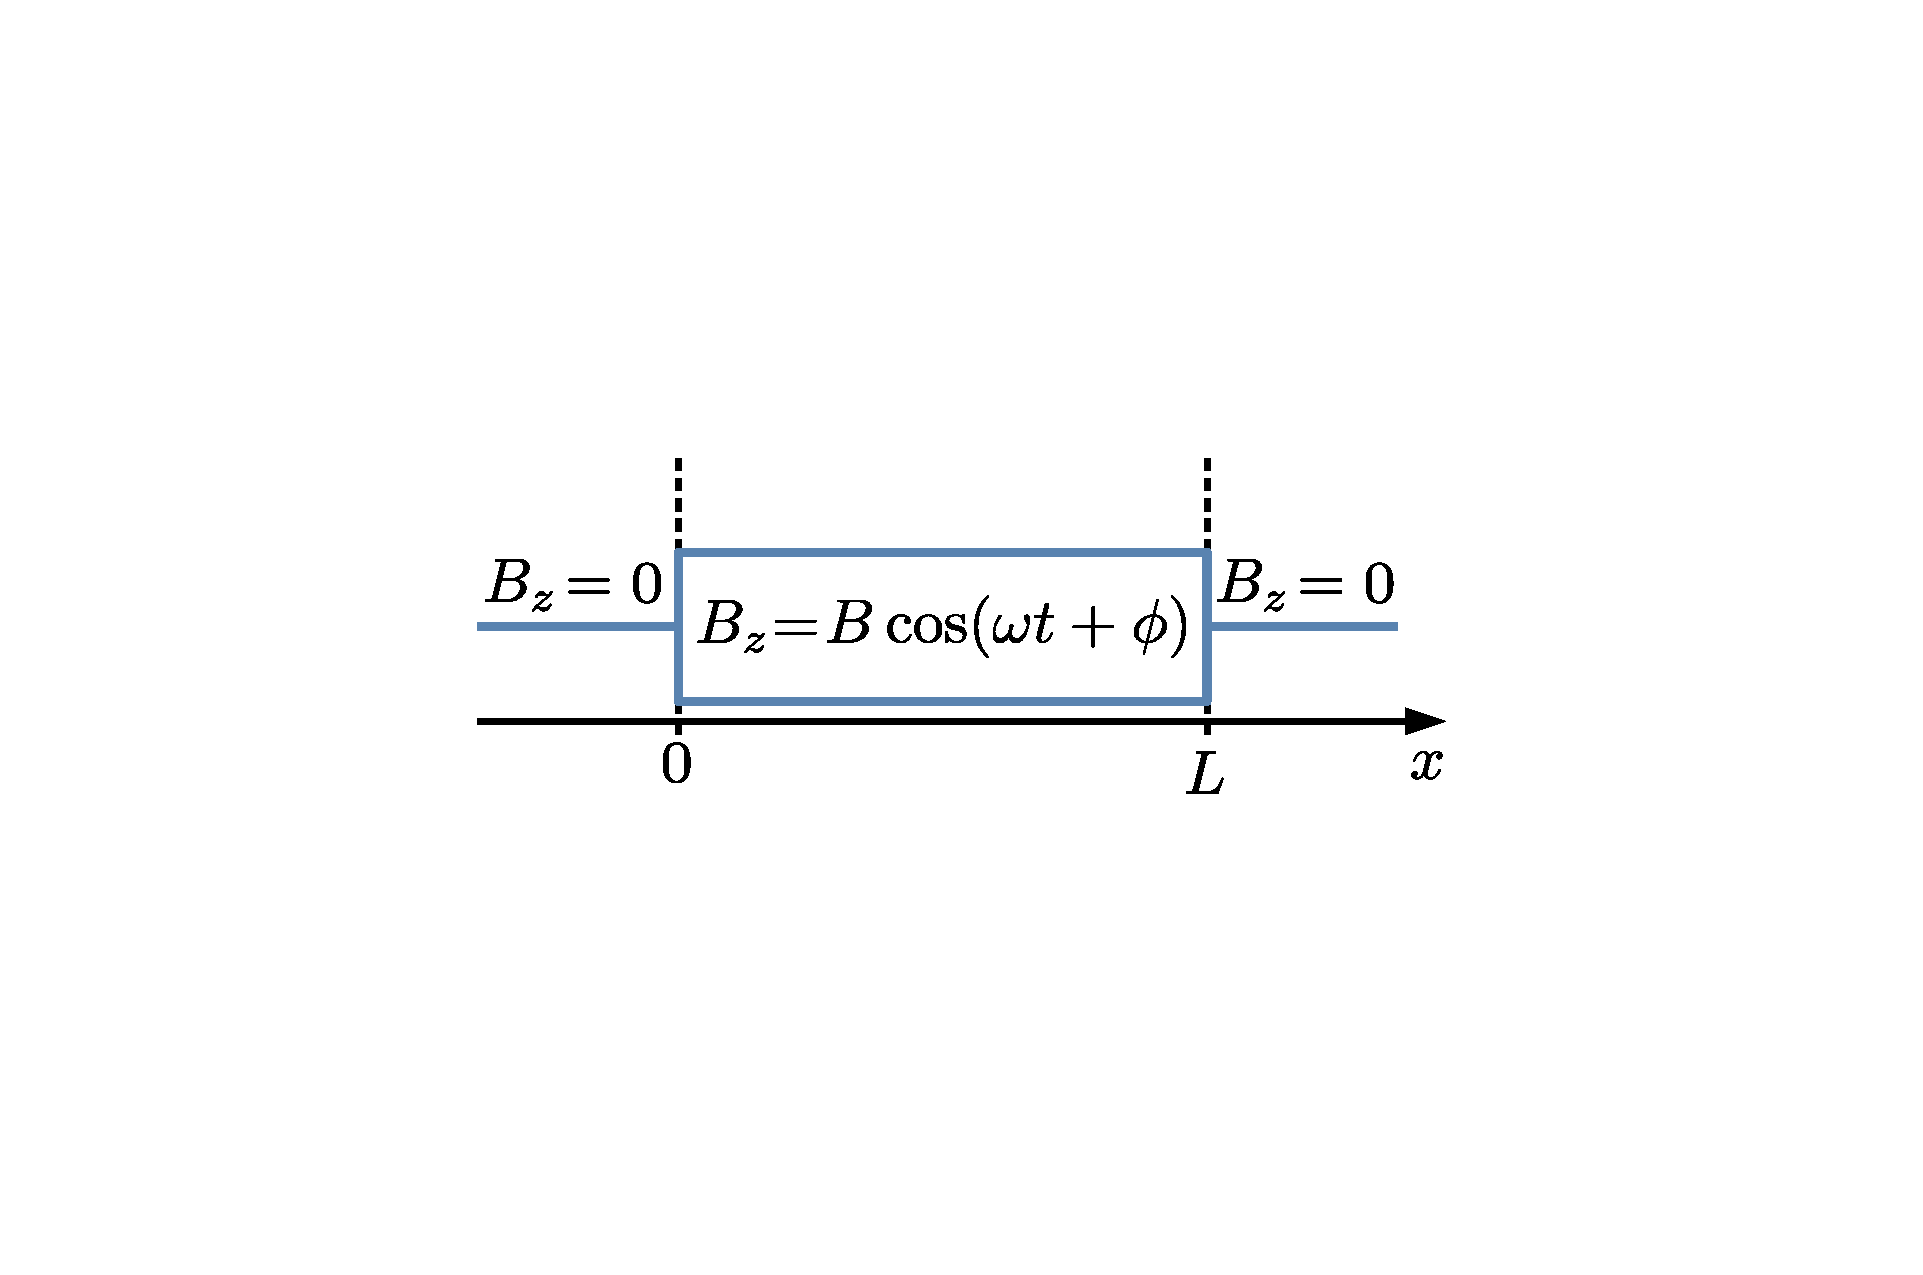
\includegraphics[width=\linewidth,trim={8cm 8cm 8cm 7cm},clip]{Magnetic field.pdf}
\caption{\label{fig:B field} Magnetic field}
\end{wrapfigure}
where $\hat{\Vec{\sigma}}=(\hat{\sigma}_x, \hat{\sigma}_y, \hat{\sigma}_z)$ is the Pauli matrices vector and $\psi(x,t)=\bra{x}\braket{\uparrow_z\rvert\psi(t)}$.
The constants $\hbar$, $m$, and $\mu$ are the reduced Planck's constant, the mass of the neutron, and the neutron magnetic moment, respectively. The SP equation can be solved for the different regions of space $x<0$, $0<x<L$, and $x>L$, and the boundary conditions at $x=0$ and $x=L$ can be used to define the wave-function.

Presenting a detailed derivation is beyond the scope of this paper, in the following only a qualitative description is reported; for a thorough derivation one can refer to \cite{summhammer1995,summhammer1993, sulyok2011, Haavig1982}. The oscillating field excites the energy levels $\omega_n=\omega_0+n\omega$ of the neutron, with $\omega_0 = \hbar k_0/2m$
being the energy of the neutron in free space. The wave-function for $x>L$ takes the form
\begin{align}
\begin{aligned}
    \psi_{x>L}(x,t) = \sum_{-\infty}^{+\infty}J_n(\alpha)\e^{-\I n \eta} \e^{\I( k_nx-\omega_n t)} \approx \e^{\I( k_0 x-\omega_0 t)} \sum_{-\infty}^{+\infty} J_n(\alpha)\e^{-\I n(\eta-\frac{m}{\hbar k_0}\omega x - \omega t )} \,,
\end{aligned} \label{eq:time phase}
\end{align}
where $J_n(\cdot)$ is the $n$-th Bessel function of the first kind, and
\begin{align}
    \alpha = 2\dfrac{\mu B}{\hbar \omega} \sin(\omega T/2)\,,\quad \eta = \varphi + \frac{\omega T+\pi}{2}, \quad k_n = \sqrt{k_0^2-\frac{2m}{\hbar}n\omega} \approx k_0 -\frac{m}{\hbar k_0}n\omega\,.
\end{align}
The parameter $T$ is the time of flight of the neutron in the region $0<x<L$, i.e the interaction time, and $m/\hbar k_0=v_0$ is the neutron velocity in free space. The approximation of $k_n$ is due to the energy of the neutron being much higher than the magnetic fields involved and, for the same reason, we can neglect reflections in the region $x<0$. Therefore, we can assume $\psi_{x<0}(x,t)=\e^{\I( k_0 x-\omega_0 t)}$ and by using the Jacobi-Anger expansion we can rewrite \eq\,\eqref{eq:time phase} as
\begin{align}
\begin{aligned}
    \psi_{x>L}(x,t) \approx \e^{\I( k_0 x-\omega_0 t)} \e^{-\I \alpha \sin(\omega t+\eta-\frac{\omega}{v_0} x)} = \psi_{x<0}(x,t) \e^{-\I \alpha \sin(\omega t+\xi)}
\end{aligned}
\end{align}
with $\xi=\varphi+(\omega T+\pi)/2-\omega x/v_0$ being a constant for a fixed detector position. In other words, the overall effect of the interaction with the oscillating magnetic field is the generation of a sinusoidal time-dependent phase.
\section{Measurements with arbitrary acquisition time}\label{app:time-avg}
The time-averaged intensity measured in the time interval $(t_1,t_2)$, with an acquisition time $\tau=t_2-t_1$, can be expressed as (see \eq\,\eqref{eq:I+-})
\begin{align}
\begin{aligned}
    \braket{I_\pm(\chi, t)}_{\tau}&=\frac{1}{\tau} \int_{t_1}^{t_2} I_\pm(\chi,t) \, \mathrm{d}t = \frac{1}{2} \pm \frac{a_1 a_2}{\tau}\int_{t_1}^{t_2} \cos(\chi+\rho_1(t) - \rho_2(t)) \, \mathrm{d}t \\
    & = \frac{1}{2} \pm \frac{a_1 a_2}{2 \tau}\int_{t_1}^{t_2} \left(\e^{\I(\chi+\rho_1(t) - \rho_2(t))} + \e^{-\I(\chi+\rho_1(t) - \rho_2(t))}\right)\,\mathrm{d}t\, ,
\end{aligned} \label{eq:int I+- app}
\end{align}
where in the last step the cosine has been expanded using Euler's formula. The exponential terms present in the integral can be rewritten using the Jacobi-Anger expansion as
\begin{align}
\begin{aligned}
    \e^{\pm \I  \rho_i(t)}&=\e^{\pm \I  \alpha_i \sin(\omega_i t+\xi_i)} = \sum_{n=-\infty}^\infty J_n(\pm\alpha_i) \e^{\I  n(\omega_i t+\xi_i)}=\sum_{n=-\infty}^\infty J_n(\alpha_i) \e^{\I  \left[\pm n(\omega_i t+\xi_i)\right]} \, ,\label{eq:bessel1}
\end{aligned}
\end{align}
with $J_n(\cdot)$ being the $n$-th Bessel function of the first kind. In the last step, the property $J_n(-x)=J_{-n}(x)$
has been used. 
Consequently, we can re-write \eq\,\eqref{eq:int I+- app} as

\begin{align}
\begin{aligned}
   \braket{I_\pm(\chi, t)}_{\tau} \, &=\frac{1}{2} \pm \frac{a_1 a_2}{2 T} \sum_{n,m=-\infty}^\infty J_n(\alpha_1)J_m(\alpha_2) \\ & \times \int_{t_1}^{t_2} \left( \e^{\I[\chi+n(\omega_1 t+\xi_1) - m(\omega_2 t+\xi_2)]} + \e^{-\I[\chi+n(\omega_1 t+\xi_1) - m(\omega_2 t+\xi_2)]}\right)\,\mathrm{d}t \,,
\end{aligned}
\end{align}
or, equivalently as
\begin{align}
\begin{aligned}
   \braket{I_\pm(\chi, t)}_{\tau} \, &= \frac{1}{2} \pm \frac{a_1 a_2}{\tau} \sum_{n,m=-\infty}^\infty J_n(\alpha_1)J_m(\alpha_2) \int_{t_1}^{t_2} \cos(\chi +\omega_{nm} t + \xi_{nm})
     \, \mathrm{d}t \,,
\end{aligned}
\end{align}
with $\omega_{nm}=n \omega_1 - m \omega_2$ and $\xi_{n,m}=n \xi_1 - m \xi_2$. In the case of only one coil being active, \eq\,\eqref{eq:int I+-} reduces too
\begin{align}
\begin{aligned}
   \braket{I_\pm(\chi, t)}_{\tau} \, &= \frac{1}{2} \pm \frac{a_1 a_2}{\tau} \sum_{n=-\infty}^\infty J_n(\alpha_i) \int_{t_1}^{t_2} \cos(\chi +n \omega_i t + n \xi_i)
     \, \mathrm{d}t \,,
\end{aligned} \label{eq:int I+- one coil}
\end{align}
with $i$ indicating the active coil. For a sufficiently long acquisition time $\tau_\infty\rightarrow\infty$, \eq\,\eqref{eq:int I+- one coil} reduces to
\begin{align}
\begin{aligned}   
    &\braket{I_\pm(\chi, t)}_{\tau\rightarrow\infty} = \frac{1}{2} \pm a_1 a_2 J_0(\alpha_i) \cos \chi \, .
\end{aligned} \label{eq:int_I+-_T_inf_app}
\end{align}
\section*{References}
\bibliographystyle{iopart-num}
\bibliography{references}% Produces the bibliography via BibTeX.
\end{document}
%
% ****** End of file apssamp.tex ******